\documentclass[../../Problems]{subfiles}
\begin{document}
\subsection{Delannoy Number}{\label{pp:delannoynumber}}
Consider a grid with $m$ horizontal lines and $n$ vertical lines. A Delannoy Number is defined as the path from bottom-left corner of the grid to the top right corner by walking along the lines \emph{or diagonally upwards}; so, the person is constrained to move only in positive $x$ or positive $y$ or positive $x-y$ (i.e. along $y=x$) direction.
\begin{figure}[H]
	\centering
	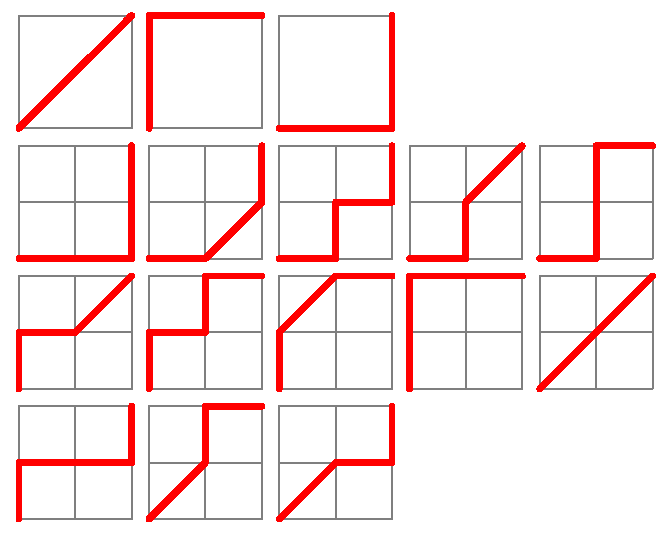
\includegraphics[width = 0.3\linewidth]{Delannoy Number.pdf}
	\caption{Example walks for case $m=n=1\ (\#2),\ m=n=2\ (\#6),\ m=n=3\ (\#20)$ (\href{https://mathworld.wolfram.com/DelannoyNumber.html}{Image Source})}
	\label{fig:delannoynumber}
\end{figure}
\vspace{-1em}
\textbf{Problem Statement:}\\
Find the number of possible \emph{Delannoy Numbers} for a given $m,n$ (for all test cases).
\begin{testcasesFunction}
	{$t$ \hfill(number of test cases, an integer)\\
	$m_1\ n_1\ \quad m_2\ n_2\ \quad \ldots\quad m_t\ n_t$ \hfill($t$ space seperated integer pairs for each testcase)}
	{Number of Delannoy Numbers for $m_i, n_i$  \hfill(each test case on a newline)}
	{$1 \leq m_i, n_i \leq 13$}
	{\texttt{int delannoy\_number(int m, int n)} -- returns the number of Delannoy Numbers for $m,n$.}
	% {6\\1 1\quad 2 5\quad 6 3\quad 7 10\quad 13 8\quad15 15}
	{11\\1 1\quad 2 2\quad 3 3\quad 5 5\quad 10 10\quad 13 13\quad 2 5\quad 3 3\quad 6 3\quad 7 10\quad 13 8}
	{3\\13\\63\\1683\\8097453\\1409933619\\61\\63\\377\\433905\\8405905}
	{https://github.com/paramrathour/CS-101/tree/main/Starter Codes/Delannoy Number.cpp}
\end{testcasesFunction}
\end{document}